\chapter{Materiais e Métodos}

Para a solução do problema de acompanhamento do crescimento de plantas, principalmente em contextos de larga escala, como grandes fazendas, os autores propõem aqui uma solução que se baseia na segmentação das imagens obtidas e extração de medidas a partir do segmento correspondente à planta.

Existem diversos algoritmos para segmentar a imagem e obter corretamente os pixels correspondentes à planta. Estratégias mais simples como a definição de um limiar para os valores aceitáveis de verde, por exemplo, podem ser aplicadas, embora sua simplicidade (e, portanto, facilidade de implementação) resulte em resultados menos adequados. Também existem técnicas mais avançadas e robustas, como o uso de algoritmos de aprendizado de máquina, cabendo aos autores fazer o treinamento desses algoritmos para obter os resultados com a precisão que desejamos. Durante a execução desse trabalho, os autores pretendem determinar qual estratégia de segmentação é a mais apropriada para os resultados desejados.

A extração de medidas, assumindo um algoritmo perfeito de segmentação, torna-se elementar. Para obter os dados da área precisamos apenas contar os pixels que existem naquele segmento. Para altura da planta, a estratégia escolhida é realizar uma regressão linear com os pontos do segmento, assim normalizando a possivel rotação da imagem, a partir do sistema de coordenadas baseado na reta obtida podemos obter os pontos máximo e mínimo no eixo Y, que correspondem à altura. Para a largura, projetamos os pontos do segmento no eixo X deste sistema de coordenadas e obtemos a distância entre os pontos máximo e mínimo, que correspondem à largura da planta.

Quanto aos materiais necessários, estes consistem simplesmente de imagens de plantas. Qualquer imagem encontrada na internet que mostre uma planta pode ser utilizada para testar a aplicação final. Além disso, pode-se fazer necessário o uso de um \textit{dataset} de imagens para o treinamento do algoritmo de aprendizado de máquina, caso esta seja a estratégia de segmentação adotada. Este deve ser composto por imagens de plantas com a segmentação já feita. Existem diversos \textit{datasets} disponíveis na internet que podem ser utilizados para esse fim.

Quanto a limitações, espera-se que, dependendo do algoritmo de segmentação escolhido, a imagem pode não ser segmentada corretamente caso existam outros elementos de cor semelhante ao verde. Outra limitação dá-se pela natureza do algoritmo de regressão linear, que dependendo da orientação da planta (mais horizontal ou vertical) pode inverter logicamente os valores de altura e largura, embora na imagem final isso seja representado de forma indiferente. Também é importante ressaltar que foge do escopo deste trabalho a conversão de medidas de pixels para medidas reais, como centímetros ou metros, uma vez que isso depende de diversos fatores como a distância da câmera em relação à planta, a qualidade da imagem, entre outros. Dado isso, para que as medidas sejam consistentes no tempo, é importante que as imagens sejam tiradas sempre da mesma distância, ângulo e condições de iluminação.

A aplicação final deve então utilizar esses algoritmos de segmentação, determinação de área, altura e largura para entregar ao usuário uma interface onde ele pode enviar as imagens de suas plantas, obtendo assim a imagem processada, composta pela imagem original com uma máscara aplicada e os dados de área, altura e largura da planta, como observado na Figura \ref{fig:exemplo-imagem-processada}.

\begin{figure}
    \centering
    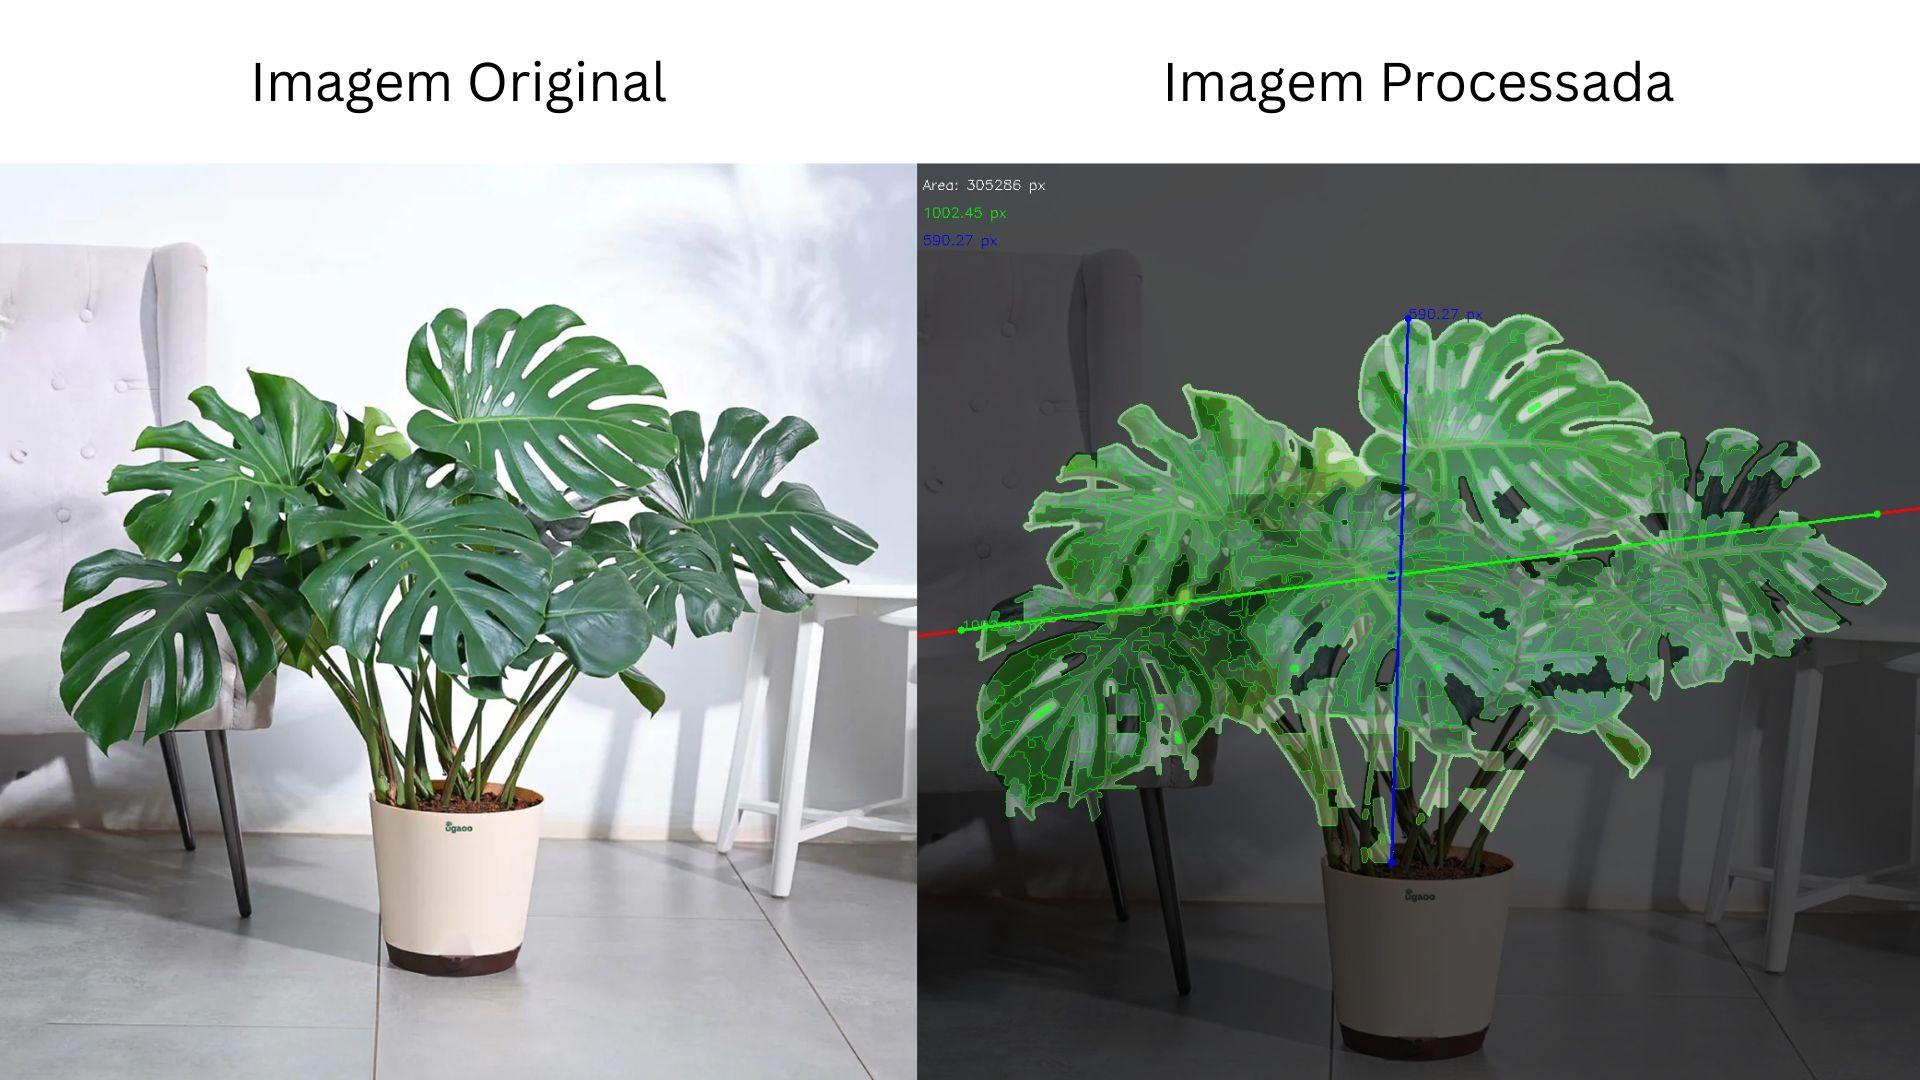
\includegraphics[width=1\textwidth]{../figures/pi/exemplo-imagem-processada.jpg}
    \caption{Imagem processada com a máscara aplicada e os dados de área, altura e largura da planta. Fonte: os autores.}
    \label{fig:exemplo-imagem-processada}
\end{figure}
